\documentclass[sigconf,nonacm]{acmart}

% links
\usepackage{hyperref}
% foreach macro
\usepackage{pgffor}
% file contents utilities
\usepackage{filecontents}
\usepackage{array}
\usepackage{subcaption}
\usepackage{graphicx}

%%
%% \BibTeX command to typeset BibTeX logo in the docs
\AtBeginDocument{%
  \providecommand\BibTeX{{%
    \normalfont B\kern-0.5em{\scshape i\kern-0.25em b}\kern-0.8em\TeX}}}

\newcolumntype{L}{>{\centering\arraybackslash}m{3cm}}

\begin{document}

\title{ThisEventDidNotHappen}
\subtitle{Data/Science/Society \\ Student ID: ge38rak \\ Winter Term 2020/2021}

\author{Adrian David Castro Tenemaya}
\email{adrian.castro@tum.de}
\affiliation{%
  \institution{Technische Universit{\"a}t M{\"u}nchen}
}

\begin{abstract}
  Even before internet became popular, fake news and people disguising themselves as someone else existed all over the world. From gossip spreading, to the use of fake passports, going ``off the grid'' and living in the woods. People always tried to get away from something they were, or something they have done, or tried to change the course of history by telling lies.

  The effect however, has been ever so slow as the fastest mean of communication available at the time.

  Communication at the speed of light is a game changer. In seconds, people across the globe know about fake cults, conspiracy theories, and much, much more.
  Today, a \textit{tweet} alone can alter the course of history, save lives, or even take them away.

  Today, people can be whoever they want online. A waitress, a business owner, a monk, or a dog. On the internet, no one knows you are a dog.

  Today, people can change their faces on the internet, or create entirely new ones, never before seen.

  Today, more than ever, pen is mightier, and faster, than the sword.
\end{abstract}

\maketitle

\section{Introduction}

Around 2014, Generative Adversarial Networks, a type of neural network designed by Ian Goodfellow and his team \cite{goodfellow2014generative}, was introduced. The next year, Batch Normalization \cite{ioffe2015batch} and the definition of Residual Networks \cite{he2015deep} was born. These, amongst many more discoveries up until today allowed neural networks to deeper, more efficiently, and with much better results.

One paper from 2015 \cite{denton2015deep} shows outstanding -- for the time -- results in terms of image generation using GANs. From a very low quality image, the network is able to generate a completely new image, either reconstructing the original, or coming up with its own interpretation of the available data (Figure \ref{fig:eyescream}). The same year, another team in Toronto developed a neural network that could generate images from a natural language text description (Figure \ref{fig:gen_attention}). This was merely the start of the GAN revolution.

GANs allow the use of parameters that can be tuned to generate specific variants of the same output image. An example is the image of the face of a person, that smiles or frowns, according to a given parameter, or turns its head left and right, or has glasses on or off.

These advancements looked great, as they served to push the advancements in the field much forward. In the following years, more and more papers regarding GANs started to show up, highlighting the immense potential that this neural network architecture provided. As the development in this field progressed, more discoveries were made, and higher quality images could be reproduced.

In the following sections we are going to discuss what is realistic image generation more in detail, why it is a problem in the modern society, and what are possible consequences.

\begin{figure}
    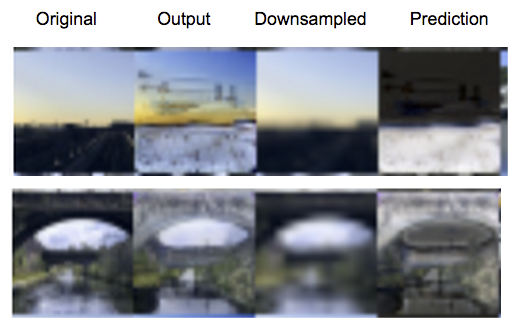
\includegraphics[width=\linewidth]{00_Introduction/eyescream_predicted16.png}
    \Description[Skyline and bridges, generated by Eyescream (2015)]{Skyline and bridges, generated by Eyescream (2015)}
    \caption{Skyline and bridges, generated by Eyescream (2015)}
    \label{fig:eyescream}
\end{figure}

\begin{figure}
    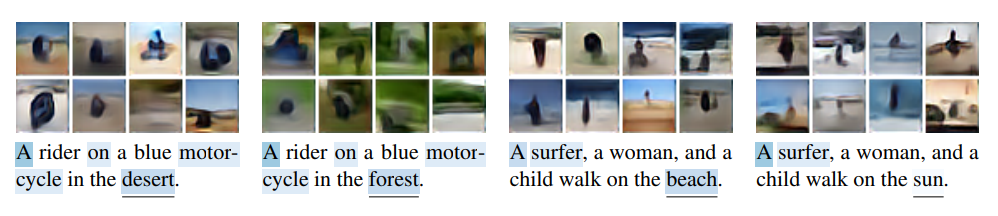
\includegraphics[width=\linewidth]{00_Introduction/gen_from_captions.png}
    \Description[Example of most attended words while changing the background in the caption]{Example of most attended words while changing the background}
    \caption{Example of most attended words while changing the background}
    \label{fig:gen_attention}
\end{figure}

\section{All Your Data Are Belong To Us}

When the internet started to become mainstream, most people didn't really understand how vulnerable their online presence was, and the same was true the other way around. Webmasters and people who owned the very first servers and windows to the internet, didn't really understand how impactful their user data could be.

The first restaurant to accept online orders was none other than Pizza Hut, in 1994, and it was one of the first 10.000 websites to hit the World Wide Web, and it used an online form to gather their customer's email and phone number information to deliver pizza. Very simple and effective.

Thirty years later on the same website you can create an account, look at a map of all the Pizza Huts in the world, look for a job, download the app, sign up for a fantastic pizza prize. And ah, yes, also order a pizza. In a relatively short amount of time, the number of additional services that website offer skyrocketed, and so has the means of tracking users.

This data is not only used to help users serve a hot, steamy pizza to their doorstep, but also to understand which kind of pizza they want the most, at specific times of the year. This data is used to track and predict where the next Pizza Hut store should be, to maximize the number of pizzas to be delivered.

Some people however, began to be highly concerned with the fact that their presence online was being used not only to satiate their appetite, but also for other means. Websites like \textit{Google} and \textit{Yahoo!} saw the potential of using user's searches through the web to show them advertisements. So suddenly, after you visit \textit{PizzaHut.com} for your midnight cravings, the next time you visit \textit{Bloomberg.com} a small box pops out, with \textit{Domino's} menu.

Over time people grew concerned and, as it always was, wanted to regain their freedom of choosing what their information was being used for.

\section{The Rise of Fake Identities}

Her name is Josie O. Campbell. She lives in Tigard, Oregon, is 45 years old and has been working as a veterinary assistant and laboratory animal caretaker for 10 years. Her car is a 1993 Mazda Lantis, and her favorite color is purple.

The previous paragraph is a description of a fake person, generated by the website \href{https://fakenamegenerator.com}{FakeNameGenerator.com}. It is a rather simple, yet effective free tool that creates a fictional person given a set of basic parameters, such as the gender, name set (American in this case, but it could have been Arabic, Hispanic or even Chinese), and country. In the past years, the need for protecting one's privacy online went up dramatically, aided by the fact that people are increasingly more conscious about their online persona, and the digital trail they might leave behind.

Internet users are using these sorts of fake accounts to sort of ``anonymize'' their presence online, by just hitting the button ``generate'' every time they visit a new website that they don't really care about, or entirely trust.

This situation has caused a lot of trouble amongst social media websites and online forums, as any suspicious or malicious activity is a lot more difficult to tackle with fake information. Because of this, platforms have become more and more active in the pursuit of the deletion of fake accounts. Facebook alone deleted 2.2 \textit{billion} of fake accounts just in the first quarter of 2019, not including the ones that didn't even get activated in the first place.

Most of us who have an account on social medias like Twitter or Instagram, have quite an experience with this kind of fake accounts. For example, you might have received a shady Instagram follow request from a young, prosperous lady with a shadier description, usually with the emoji ``Adults only'', some cucumbers and hearts. Or perhaps you might have heard that your coworker wants to see if his fiancé is loyal, and has created a fake account to go and take a shot to his significant other.

Indeed, there are legitimate uses for fake accounts. To preserve one's identity, to innocently (or not) spying on other people's lives, or to simply please your mother with an Instagram where you just post your best panorama pictures.

However, the problem comes with the fake, automatically created accounts. Their use varies widely, as we previously pointed out, with most of them being used for financial profit. This is not true however for another category of malicious, and potentially more dangerous acts: fake news spreading.

\begin{figure}
    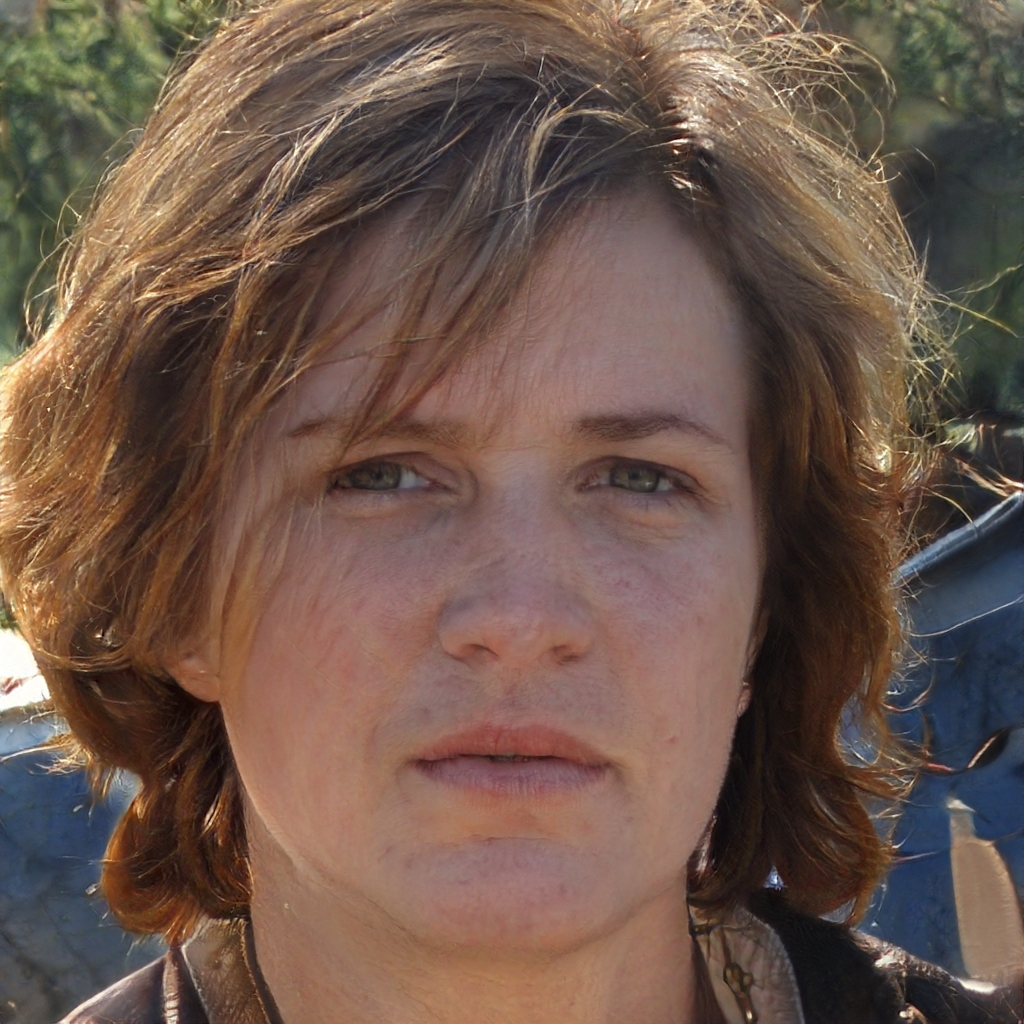
\includegraphics[width=0.5 \linewidth]{02_RiseOfFakeIdentities/image.jpg}
    \caption{Josie O. Campbell: a fake person generated by an AI}
    \label{fig:fakeperson}
\end{figure}

\section{Fake News}

You might have subscribed to online news magazines from time to time, and read through their articles. They might not look different at all from the ones that we see in real life, except from the fact that they are written on pixels on screen instead of ink on paper. Even the titles sound the same: ``Godzilla Invaded New York!'', ``President Shaking Hands With Pope'', ``Winter Is Coming: Buy BrandName''.

However, titles, \textit{recommendations} that you see and the articles that you read, evolved along with the algorithms that show them to you. This became overtime one of the most debated arguments of how the internet works, and how companies make money. On YouTube for example, content creators have to keep track of every algorithm change, leading to the fact that everything they create, is not actually done to appease the users, but to appease the algorithm. If you don't show in people's recommendations, you don't exist.

Titles, thumbnails, video length, sponsors, advertisements. Everything has to be done in such a way that the algorithm favors your videos amongst a million other. Of course, this also applies everywhere a content creator posts their content, such as Google, Instagram, LinkedIn or Twitter. This is why it is more and more common to see titles such as: ``HOW TO BECOME A BIRD IN 10 STEPS'', ``JOKE: BIG BALL HITS PEOPLE, PRANK!'' and thumbnails with bright, saturated pictures of people with their mouths open in awe, and some dollar bill signs, because why not.

Of course, this is not entirely to blame to algorithms. We as users click on those articles and videos, basically telling the underlying system that yes, this system works, and we want to see that video and watch it to the end. This is how the internet uses algorithms to hack human nature.

This ``hack'' can in turn be used to manufacture articles in such a way that people are guaranteed to take a look at them, starting from the title. As an example, using ``Pope Francis Meets Donald Trump'' is much less effective in gaining clicks than ``Pope Francis Shocks The World, Endorses Donald Trump for President''. Although untrue, the latter is far more likely to be seen in social media, to get clicked on and to get shared amongst peers. In turn, this generates revenue for the article poster, via clicks on advertisement banners, which usually proliferate on their websites like shrooms in a forest.

You might have had the misfortune to find somebody in your life that shared some of these kind ``clickbaity'' of articles to you, or to their social media pages, like their \textit{wall} on Facebook or as a \textit{tweet} on Twitter. What I call misfortune is confronting them on the truthfulness of said article, and failing to making their posters to admit that they were wrong about believing that Elizabeth, Queen of England, is actually just a pawn of a secret group called the ``World Order''.

What happened there? Why did your friend start to believe in such stories, and why? Well, as it always has been, when enough people start to believe in something, that belief becomes reality. An untrue one, but an alternative reality nonetheless.

The same thing can be said for example about Galileo Galilei, the scientist who in 1609 defended his position of heliocentrism based on his astronomical observations in front of a jury of a very Christian jury. At that time, the occidental world lived within an alternative reality, where the earth is at the center of the universe, and the Earth was flat.

This happened because enough people believed that heliocentrism was a foolish idea, based on the Bible.

What if the same thing happened today? We are in an era when ideas and opinions can go far and wide, in the blink of an eye. News, fake or true, can be told by anyone anywhere, in any position of power, for whatever reason.

Election results can suddenly change with a few tweets, trends emerge with a few viral videos on TikTok, and vaccines and a global pandemic that kills hundreds of thousands of people suddenly becomes a hoax.

\section{Bots vs GANs}

Around 2014, Generative Adversarial Networks, a type of neural network designed by Ian Goodfellow and his team \cite{goodfellow2014generative}, was introduced. The next year, Batch Normalization \cite{ioffe2015batch} and the definition of Residual Networks \cite{he2015deep} was born. These, amongst many more discoveries up until today allowed neural networks to deeper, more efficiently, and with much better results.

One paper from 2015 \cite{denton2015deep} shows outstanding --for the time-- results in terms of image generation using GANs. From a very low quality image, the network is able to generate a completely new image, either reconstructing the original, or coming up with its own interpretation of the available data (Figure \ref{fig:eyescream}). The same year, another team in Toronto developed a neural network that could generate images from a natural language text description (Figure \ref{fig:gen_attention}). This was merely the start of the GAN revolution.

GANs allow the use of parameters that can be tuned to generate specific variants of the same output image. An example is the image of the face of a person, that smiles or frowns, according to a given parameter, or turns its head left and right, or has glasses on or off.

These advancements looked great, as they served to push the advancements in the field much forward. In the following years, more and more papers regarding GANs started to show up, highlighting the immense potential that this neural network architecture provided. As the development in this field progressed, more discoveries were made, and higher quality images could be reproduced.

In the following sections we are going to discuss what is realistic image generation more in detail, why it is a problem in the modern society, and what are possible consequences.


\bibliographystyle{ACM-Reference-Format}
\bibliography{references}

\end{document}
